\documentclass[a4paper,11pt]{article}
\usepackage{booktabs} % Provides professional-quality horizontal rules
\usepackage{float} % Required for [H] placement
\usepackage{tikz} 
\author{Hectron} 
\title{3 Sum}

\begin{document}

% generates the title
\maketitle

% insert the table of contents
\tableofcontents

% seperate body and table of contents 
\newpage

\section{Description}
Given an array nums of n integers, return an array of \textbf{all the unique quadruplets}: [nums[a], nums[b], nums[c]]  such that: 

\begin{itemize}
  \item 0 <= a, b, c, d < n
  \item a, b, c, and d are distinct.
  \item nums[a] + nums[b] + nums[c] + nums[d] == target

\end{itemize}

\section{Function/Method Declaration}
\footnotesize
std::vector< std::vector<int> > threeSums(std::vector \textbf{numbers}, int target);

\section{Solution}
\begin{itemize}
    \item [I.]  Mix \textbf{numbers} with itself to find all pair combinations.
    \item [II.]  Recent sum pairs produced are crossed with \textbf{numbers} to produce another list of pairs.
    \item [III.] II is repeated N-2 times (i.e. N=4; 2 iterations)
\end{itemize}

    \subsection{First pairs}
    \noindent
    Method below is used to find unique pairs of two equal vectors (i.e. autocorrelation sampless). 

    \subparagraph{} 
    Raw vector: 
    numbers = [ 0, -4, 3, 1, 0 ] 
    
    \subparagraph{} 
    Sort set:  
    numbers = [ -4, 0, 0, 3, 3 ] 
    
    \subparagraph{} 
    Unqiue values in vector:
    numbers = [ -4, 0, 1, 3 ]
    
    \subparagraph{} 
    Pairs (diagonal search): 

\vspace*{-1\baselineskip} % Pulls text up by one line

\begin{table}[ht]
    \centering
    \caption {Sums}
    \begin{tabular}{c c c c c}
        \toprule
        \textbf{ List} & \tiny{-4} & \tiny{0}   & \tiny{1}  & \tiny{3} \\ 
        \midrule
        \tiny{-4}  &  \textbf{-8}  & {\footnotesize -4} &  {\footnotesize -3} & {\footnotesize-1 }  \\ 
        \tiny{0}   &  \textbf{-4}  & \textbf{0}  &  {\footnotesize 1}  &  {\footnotesize{3}  } \\ 
        \tiny{1}   &  \textbf{3 }  & \textbf{1}  &  \textbf{2}  &  {\footnotesize{4} }  \\ 
        \tiny{3}   &  \textbf{-1}  & \textbf{3}  &  \textbf{4}  &  \textbf{3}    \\ 
        \bottomrule
    \end{tabular}
\end{table}
    
    
    \newpage

    \noindent
    
    \subsection{Other pairs}

    \paragraph{} 
    
    Method below is used to find unique pairs of input vector with previous sum pairs:

    \subparagraph{} 
    Input set: numbers = [ -4, 0,  1, 3 ] 
    
    \subparagraph{} 
    Sums set: numbers = [ -8, -4, -1, 0, 1, 2, 3, 4 ] 

    \begin{table}[ht]
        \centering
        \caption {Sums}
        \begin{tabular}{c c c c c  }
            \toprule
            \textbf{ List}  & \tiny{-4}         & \tiny{0}              & \tiny{1}                  & \tiny{3} \\                   \\
            \midrule    
            \tiny{-8}       &   \textbf{-12}    & {\footnotesize -8}    &  {\footnotesize -7}       & {\footnotesize-5 }            \\ 
            \tiny{-4}       &   \textbf{-8}     & \textbf{-4}           &  {\footnotesize -3}       &  {\footnotesize{-1}  }         \\ 
            \tiny{-1}       &   \textbf{-5}     & \textbf{-1}           &  \textbf{0}               &  {\footnotesize{2} }          \\ 
            \tiny{0}        &   \textbf{-4}     & \textbf{0}            &  \textbf{1}               &  \textbf{3}                   \\ 
            \tiny{1}        &   \textbf{-3}     & \textbf{1}            &  \textbf{2}               &  \textbf{4}                   \\ 
            \tiny{2}        &   \textbf{-2}     & \textbf{2}            &  \textbf{3}               &  \textbf{5}                   \\ 
            \tiny{3}        &   \textbf{-1}     & \textbf{3}            &  \textbf{4}               &  \textbf{6}                   \\ 
            \tiny{4}        &   \textbf{0 }     & \textbf{4}            &  \textbf{5}               &  \textbf{7}                   \\ 

            \bottomrule
        \end{tabular}
    \end{table}

        
    \subsection{FlowChart}
        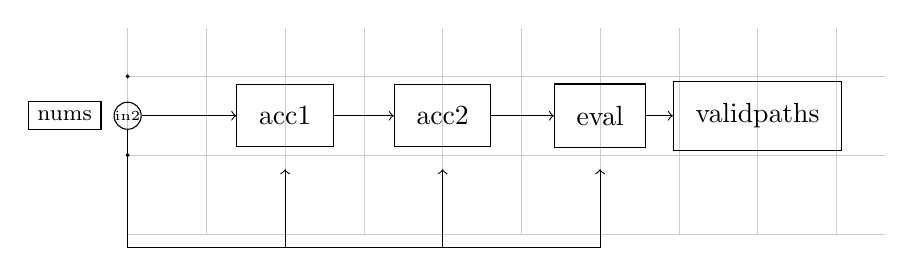
\begin{tikzpicture}[node distance=1.5cm]

        \draw[help lines, opacity=0.4] (0,0) grid (10,3, );
        
        % Define nodes (boxes)

        \node (in)  at ( -0.8, 1.5) [draw, font=\fontsize{8}{10}\selectfont ] {nums};

        \node (in2) at (0, 1.5) [circle , draw, minimum size=2pt, inner sep=0pt, font=\fontsize{2}{4}\selectfont ] {in2};

        \node (acc1) at ( 2.0, 1.5 ) [rectangle , draw, minimum size=4pt, inner sep=8pt] {acc1};
        
        \node (acc2) at ( 4.0, 1.5 ) [rectangle , draw, minimum size=4pt, inner sep=8pt] {acc2};
        
        % \node (acc3) at ( 6.0, 1.5 ) [rectangle , draw, minimum size=4pt, inner sep=8pt] {acc3};

        \node (eval) at ( 6.0, 1.5 ) [rectangle , draw, minimum size=4pt, inner sep=8pt] {eval};
        
        \node (validpaths) at ( 8.0, 1.5 ) [rectangle , draw, minimum size=4pt, inner sep=8pt] {validpaths};


        % \node {acc2} ( 6.0, 1.5 ) [rectangle , draw, minimum size=4pt, inner sep=8pt] {acc2};

        \node (a) at ( 0.0, 1.0 ) [ circle, draw, fill, minimum size=1pt, inner sep=0pt ]{ }; 
        
        \node (b) at ( 0.0, 2.0 ) [ circle, draw, fill, minimum size=1pt, inner sep=0pt ]{ }; 

        % \node (step3) [rectangle, draw, below of=step2] {End};

        % Draw arrows between nodes

        \draw[->] (in2) -- (acc1);

        % \draw[->] (in2) -- (a);
        

        \draw[->] (in2.south) -- ++(0, -1.5)  -- ++(2.0, 0.0) -- ++(0.0, 1.0)  ;

        \draw[->] (in2.south) -- ++(0, -1.5)  -- ++(4.0, 0.0) -- ++(0.0, 1.0)  ;

        \draw[->] (in2.south) -- ++(0, -1.5)  -- ++(6.0, 0.0) -- ++(0.0, 1.0)  ;
        
        \draw[->] (acc1) -- (acc2);

        % \draw[->] (acc2) -- (acc3);

        \draw[->] (acc2) -- (eval);

        \draw[->] (eval.east) + (0, 0) -- ++(0.0, 0)  -- (validpaths) ;

    \end{tikzpicture}



\end{document}

% numbers = [ -8, -4, -1, 0, 1, 2, 3 ]
